% !TEX root = standalone.tex


\section{Design Problems}
\label{sec:Design-Problems}

We start by defining a ``design problem with implementation'', which is a tuple of ``\F{functionality} space'', ``\Icol{implementation} space'', and ``\R{resources} space'', together with two maps that describe the feasibility relations between these three spaces (\cref{fig:setup}).

\begin{definition}
    \label{def:DPI}
    A \emph{\iindex{design problem with implementation}} (DPI) is a tuple
    \begin{equation*}
        \tup{\funsp, \ressp, \impsp, \prov,\req}
    \end{equation*}
    where:

    \begin{itemize}
        \item $\funsp$ is a poset, called \emph{\Fcol{functionality} space};
        \item $\ressp$ is a poset, called \emph{\Rcol{requirements} space};
        \item $\impsp$ is a set, called \emph{\Icol{implementation} space};
        \item the map~$\prov\colon\impsp\rightarrow\funsp$
        maps an implementation to the functionality it provides;
        \item the map~$\req\colon\impsp\rightarrow\ressp$
        maps an implementation to the resources it requires.
    \end{itemize}

    \begin{figure}[h]
        \begin{center}
            \includegraphics[scale=0.4]{gmcdp_setup}
        \end{center}
        \caption{\label{fig:setup}}
    \end{figure}
    \todo{Redo figure with consistent style, change resources to requirements,
        eval/exec to requires/provides.}
\end{definition}


A graphical notation will help reasoning about composition. A DPI is represented as a box with~$\dpinumf$ green edges and~$\dpinumr$ red edges~(\cref{fig:dp_graphical}).

\begin{figure}[h]
    \centering
    \includesag{520_general_dp}
    \caption{\label{fig:dp_graphical}}
\end{figure}

%\captionsideleft{\label{fig:dp_graphical}}{\includegraphics[scale=0.33]{gmcdp_dp_graphical.pdf}}

This means that the functionality and resources spaces can be factorized in~$\dpinumf$ and~$\dpinumr$ components: $\funsp=\prod_{i=1}^{\dpinumf}\pi_{i}\funsp_{i},$
$\ressp=\prod_{j=1}^{\dpinumr}\pi_{j}\ressp$, where ``$\pi_{i}$''
represents the projection to the $i$-th component. If there are no
green (respectively, red) edges, then $\dpinumf$ (respectively, $\dpinumr$)
is zero, and $\funsp$ (respectively, $\ressp$) is equal to~$\One=\{\left\langle \right\rangle \}$,
the set containing one element, the empty tuple~$\left\langle \right\rangle $.

These \emph{co-design diagrams} are not to be confused with signal
flow diagrams, in which the boxes represent oriented systems and the
edges represent signals.


\begin{example}
    We now want to revisit the leading example of \cref{sec:attributes_sameness} with the newly introduced co-design perspective. Let's consider a list of electrical motors as in~\cref{tab:electric_motors_2}.
    \begin{table}[h]
        \centering
        \adjustbox{max width=\textwidth}{%
            \begin{tabular}{c|c|c|c|c|c}
                Motor ID & Company & $\unit[\text{Torque}]{[kg\cdot cm]}$ & \unit[Weight]{[g]} & \unit[Max Power]{[W]}
                & \unit[Cost]{[USD]}
                \\
                \hline
                \textsf{1204} & \textsf{SOYO}        & 0.18 & 60.0  & 2.34 & 19.95  \\
                \textsf{1206} & \textsf{SOYO}        & 0.95 & 140.0 & 3.00 & 19.95  \\
                \textsf{1207} & \textsf{SOYO}        & 0.65 & 130.0 & 2.07 & 12.95  \\
                \textsf{2267} & \textsf{SOYO}        & 3.7  & 285.0 & 4.76 & 16.95  \\
                \textsf{2279} & \textsf{Sanyo Denki} & 1.9  & 165.0 & 5.40 & 164.95 \\
                \textsf{1478} & \textsf{SOYO}        & 19.0 & 1,000 & 8.96 & 49.95  \\
                \textsf{2299} & \textsf{Sanyo Denki} & 2.2  & 150.0 & 5.90 & 59.95
            \end{tabular}%
        }
        \caption{A simplified catalogue of motors.}
        \label{tab:electric_motors_2}
    \end{table}

    We can think of this as a catalogue of electric motors~$\tup{\impsp_\mathrm{EM},\prov_\mathrm{EM},\req_\mathrm{EM}}$. In particular, the set of implementations collects all the motor models, which we can specify using the motor IDs:
    \begin{equation}
        \impsp_\mathrm{EM}=\{1204,1206,1207,2267,2279,1478,2299 \}.
    \end{equation}
    We now have to think about \R{resources} and \F{functionalities}. Each motor \R{requires} some \R{weight} (in \unit[]{g}), \R{power} (in \unit[]{W}), and has some \R{cost} (in USD), and \F{provides} some \F{torque} (in~$\unit[]{kg\cdot cm}$). Thus, we can identify
    \begin{equation*}
        \F{F}=\reals\times \{\unit[]{kg\cdot cm}\},\quad \R{R}=(\reals\times \{\unit[]{g}\})\times (\reals\times \{\unit[]{W}\})\times (\reals\times \{\unit[]{USD}\}),
    \end{equation*}
    by considering the units as discussed in \cref{sec:currency_cat}. The correspondences are given by the details in \cref{tab:electric_motors_2}. For instance, we have
    \begin{equation}
        \prov_\mathrm{EM}(1204)=0.18, \quad \req_\mathrm{EM}(1204)=\tup{\unit[60]{g},\unit[2.34]{W},\unit[19.95]{USD}}.
    \end{equation}
    The catalogue induces a design problem $d_\mathrm{EM}$ with diagrammatic form as in \cref{fig:dp_em}. In particular, we can query the design problem for combinations of \F{functionalities} and \R{resources}. For instance:
    \begin{equation}
        d\left(\unit[0.2]{kg\cdot cm}, \tup{\unit[50.0]{g},\unit[2.0]{W},\unit[15.0]{USD}} \right)=\false,
    \end{equation}
    since no listed model can provide~$\unit[0.2]{kg\cdot cm}$ \F{torque} by requiring the set of \R{resources} $\tup{\unit[50.0]{g},\unit[2.0]{W},\unit[15.0]{USD}}$ or less.

    \begin{figure}[tbh]
        \begin{center}
            \begin{tikzpicture}[DP]
                \node[dp={1}{3}] (mot) {Electric motor};
                \draw[runconn, runame={\R{weight}}] (mot_res1){};
                \draw[runconn, runame={\R{max power}}] (mot_res2){};
                \draw[runconn, runame={\R{cost}}] (mot_res3){};
                \draw[funconn, funame={\F{torque}}] (mot_fun1){};
            \end{tikzpicture}
        \end{center}
        \caption{Electric motor design problem.}\label{fig:dp_em}
    \end{figure}

    \begin{figure}[tbh]
        \begin{center}
            \begin{tikzpicture}[DP]
                \node[dp={2}{3}] (bat) {Battery};
                \draw[runconn, runame={$c_\mathrm{b}$}] (bat_res1){};
                \draw[runconn, runame={$m_\mathrm{b}$}] (bat_res2){};
                \draw[runconn, runame={$R_\mathrm{b}$}] (bat_res3){};
                \draw[funconn, funame={$C_\mathsf{prov}$}] (bat_fun1){};
                \draw[funconn, funame={$M_\mathsf{b}$}] (bat_fun2){};
            \end{tikzpicture}
        \end{center}
        \caption{The battery design problem.}
        \label{fig:dp_battery}
    \end{figure}

    \begin{table}[tbh]
        \begin{center}
            \begin{tabular}{cccc}
                Technology & Specific energy [\unitfrac[]{J}{kg}] & Specific cost [\unitfrac[]{J}{\$}]
                & Life [\# cycles]
                \\
                \hline
                $\mathsf{NiMH}$  & 100.0 & 3.41 & 500    \\
                $\mathsf{NiH2}$  & 45.0  & 10.5 & 20,000 \\
                $\mathsf{LCO}$   & 195.0 & 2.84 & 750    \\
                $\mathsf{LMO}$   & 150.0 & 2.84 & 500    \\
                $\mathsf{NiCad}$ & 30.0  & 7.50 & 500    \\
                $\mathsf{SLA}$   & 30.0  & 7.00 & 500    \\
                $\mathsf{LiPo}$  & 250.0 & 2.50 & 600    \\
                $\mathsf{LFP}$   & 90.0  & 1.50 & 1,500
            \end{tabular}
        \end{center}
        \caption{Specifications of common battery technologies~\cite{censi2015}. }
        \label{tab:battery}
    \end{table}
    \todo{finish with design problem description}

\end{example}




\begin{example}[Motor design]
    \label{exa:motor}Suppose we need to choose a motor for a robot from
    a given set. The \emph{functionality} of a motor could be parametrized
    by \F{torque} and \F{speed}. The \emph{resources} to consider
    could include the \R{cost {[}\${]}}, the \R{mass {[}g{]}}, the
    input \R{voltage {[}V{]}}, and the input \R{current {[}A{]}}.
    The map~$\prov:\impsp\rightarrow\funsp$ assigns to each motor its
    functionality, and the map~$\req:\impsp\rightarrow\ressp$ assigns
    to each motor the resources it needs~(\cref{fig:motor_evalexec}).
\end{example}

\begin{figure}[h]
    \centering
    \includegraphics[scale=0.4]{gmcdp_motor_evalexec}
    \caption{}
    \label{fig:motor_evalexec}
\end{figure}
\todo{Redo figure with consistent style}
%\captionsideleft{\label{fig:motor_evalexec}}{\includegraphics[scale=0.33]{gmcdp_motor_evalexec}}


\begin{example}[Chassis design]
    \label{exa:chassis}Suppose we need to choose a chassis for a robot~(\cref{fig:gmcdp_chassis_eval}).
    The implementation space~$\impsp$ could be the set of all chassis
    that could ever be designed (in case of a theoretical analysis), or
    just the set of chassis available in the catalogue at hand (in case
    of a practical design decision). The functionality of a chassis could
    be formalized as ``the ability to transport a certain \F{payload
            {[}g{]}}'' and ``at a given \F{speed {[}m/s{]}}''. More refined
    functional requirements would include maneuverability, the cargo volume,
    etc. The resources to consider could be the \R{cost {[}\${]}} of
    the chassis; the total mass; and, for each motor to be placed in the
    chassis, the required \R{speed {[}rad/s{]}} and \R{torque {[}Nm{]}}.
\end{example}
\begin{figure}[h]
    \centering
    \includegraphics[scale=0.4]{gmcdp_chassis_eval}
    \caption{}
    \label{fig:gmcdp_chassis_eval}
\end{figure}
\todo{Redo figure with consistent style}
%\captionsideleft{\label{fig:gmcdp_chassis_eval}}{\includegraphics[scale=0.33]{gmcdp_chassis_eval.pdf}}

\subsection{Mechatronics}

% $A^{\op} \profto B \to \Set$

Many mechanisms can be readily modeled as relations between a provided
functionality and required resources.


\begin{example}
    The \F{functionality} of a DC motor~(\cref{fig:dc_motor})
    is to provide a certain \F{speed} and \F{torque}, and the \R{resources}
    are \R{current} and \R{voltage}.
\end{example}

\begin{figure}[h]
    \begin{center}
        \includesag{520_dc_motor}
    \end{center}
    \caption{}
    \label{fig:dc_motor}
\end{figure}


\begin{example}
    A gearbox (\cref{fig:gearbox}) provides a certain \F{output
    torque $\tau_o$} and \F{speed $\tau_o$}, given a certain
    \R{input torque $\tau_i$} and \R{speed $\omega_i$}. For
    an ideal gearbox with a reduction ratio $r \in \ratnumbers_+$ and
    efficiency ratio $\gamma$, $0<\gamma<1$, the constraints among
    those quantities are ${\colR \omega_i}\geq r\,{\colF \omega_o}$
    and ${\colR \tau_i\omega_i}\geq\gamma\,{\colF \tau_o\omega_o}.$
\end{example}

\begin{figure}[h]
    \begin{center}
        \includesag{520_dp_gearbox}
    \end{center}
    \caption{}
    \label{fig:gearbox}
\end{figure}


\begin{example}
    \emph{Propellers}~(\cref{fig:propeller}) generate \F{thrust}
    given a certain \R{torque} and \R{speed}.
\end{example}

\begin{figure}[h]
    \begin{center}
        \includesag{520_dp_propellers}
    \end{center}
    \caption{\label{fig:propeller}}
\end{figure}

\begin{example}
    A \emph{crank-rocker} (\cref{fig:crack}) converts \R{rotational
    motion} into a \F{rocking motion}.
\end{example}

\begin{figure}[h]
    \centering
    \includesag{520_crank}
    \caption{\label{fig:crack}}
\end{figure}

\subsection{Geometrical constraints}

Geometrical constraints are examples of constraints that are easily
recognized as monotone, but possibly hard to write down in closed
form.

\begin{example}[Bin packing]
    Suppose that each internal component occupies a volume
    bounded by a parallelepiped, and that we must choose the minimal enclosure
    in which to place all components~(\cref{fig:packing}). What
    is the minimal size of the enclosure? This is a variation of the \emph{bin
    packing} problem, which is in NP for both 2D and 3D~\cite{lodi02two}.
    It is easy to see that the problem is monotone, by noticing that,
    if one the components shapes increases, then the size of the enclosure
    cannot shrink.
\end{example}

\begin{figure}[h]
    \centering
    
\includegraphics[scale=0.33]{reits2_fit_boxes}
    \caption{\label{fig:packing}}
\end{figure}
\todo{Add pics as res/fun}

\subsection{Inference}

Many inference problems have a monotone formalization, taking the
\F{accuracy} or \F{robustness} as functionality, and \R{computation}
or \R{sensing} as resources. Typically these bounds are known in
a closed form only for restricted classes of systems, such as the
linear/Gaussian setting.

\begin{example}
(SLAM)
    One issue with particle-filter-based estimation procedures,
    such as the ones used in the popular GMapping~\cite{grisetti07improved}
    method, is that the filter might diverge if there aren't enough particles.
    Although the relation might be hard to characterize, there is a monotone
    relation between the \F{robustness} (1 - probability of failure),
    the \F{accuracy}, and the \R{number of particles}~(\cref{fig:gmapping}).
\end{example}

\begin{figure}[h]
    \centering
    \includesag{520_mapping}
    \caption{\label{fig:gmapping} }
\end{figure}



\begin{example}
(Stereo reconstruction)
    Progressive reconstruction system (e.g.,~\cite{locher16progressive}),
    which start with a coarse approximation of the solution that is progressively
    refined, are described by a smooth relation between the \F{resolution}
    and the \R{latency} to obtain the answer~(\cref{fig:progressive}).
    A similar relation characterizes any anytime algorithms in other domains,
    such as robot motion planning.
\end{example}


\begin{figure}[h]
    \centering
    \includesag{520_stereo}
    \caption{\label{fig:progressive}}
\end{figure}


\begin{example}
    The empirical characterization of the monotone relation between \F{the
    accuracy of a visual SLAM solution} and \R{the power consumption}
    is the goal of recent work by Davison and colleagues~\cite{nardi15introducing,zia16comparative}.
\end{example}

\todo{Reproduce plot from paper.}

\subsection{Communication}

\begin{example}[Transducers]
    Any type of "transducer" that bridges between different
    mediums can be modeled as a DP. For example, an access point~(\cref{fig:accesspoint})
    provides the \F{"wireless access"} functionality, and requires
    that the infrastructure provides the \R{"Ethernet access"} resource.
\end{example}


\begin{figure}[h]
    \centering
    \includesag{520_ethernet}
    \caption{\label{fig:accesspoint}}
\end{figure}

\begin{example}[Wireless link]
    The basic functionality of a wireless link is to provide
    a certain \F{bandwidth} (\cref{fig:networklink}). Further refinements could include bounds
    on the latency or the probability that a packet drop is dropped. Given
    the established convention about the the preference relations for
    functionality, in which a \emph{lower} functionality is "easier"
    to achieve, one needs to choose "\F{\emph{minus} the latency}"
    and "\F{\emph{minus} the packet drop probability}" for them
    to count as functionality. As for the resources, apart from the \R{transmission
    power [W]}, one should consider at least \R{the spectrum occupation},
    which could be described as an interval $[f_0,f_1]$ of the frequency
    axis $\Runit{Hz}$. Thus the resources space is $\ressp=\colR\Runit{W}\times\aword{intervals}(\Runit{Hz})$.
\end{example}

\begin{figure}[h]
    \begin{center}
        \includesag{520_dp_wireless}
    \end{center}
    \caption{ \label{fig:networklink}}
\end{figure}

\subsection{Multi-robot systems}

In a multi-robot system there is always a trade-off between the number
of robots and the capabilities of the single robot.
\begin{example}
    Suppose we need to create a swarm of agents whose functionality is
    \F{to sweep an area}. If the functionality is fixed, one expects
    a three-way trade-off between the three resources: number of agents,
    the speed of a single agent, and the execution time. For example,
    if the time available decreases, one has to increase either the speed
    of an agent or the number of agents~(\cref{fig:multirobot2}).
\end{example}

\begin{figure}[h]
    \subfloat[]{
        \includegraphics[scale=0.33]{reits2_multirobot}

    }
    \subfloat[\label{fig:multirobot2}]{
        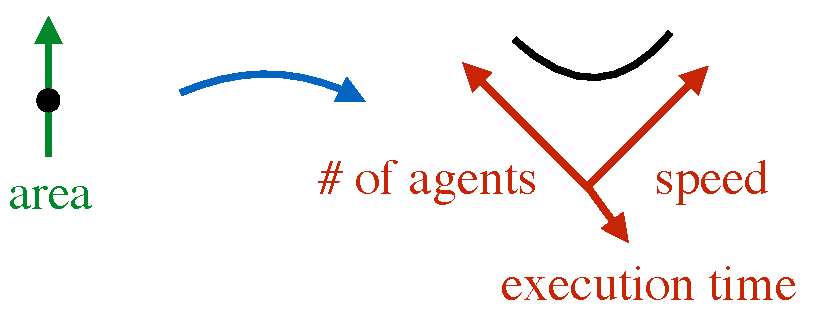
\includegraphics[scale=0.33]{reits2_multirobot2}

    }
    \caption{}
\end{figure}

\todo{redo in tikz}

\subsection{LQG Control}

\todo[inline]{Write short summary}

\subsection{Computation}


The trivial model of a CPU is as a device that provides \Fcol{computation,
    measured in flops}, and requires \Rcol{power [W]}. Clearly there
is a monotone relation between the two.

\begin{figure}[h]
    \begin{center}
        \includesag{520_dp_cpu}
    \end{center}
    \caption{}
\end{figure}

A similar monotone relation between application requirements and computation
resources holds in a much more general setting, where both application
and computation resources are represented by graphs. This will be
an example of a monotone relation between nontrivial partial orders.

In the Static Data Flow (SDF) model of computation~\cite[Chapter 3]{sriram00,lee10},
the application is represented as a graph of procedures that need
to be allocated on a network of processors.

\todo{Make the three small wrapped figures as 3 subfigures in the same figures}
% keep wrapped
\begin{wrapfigure}{r}{0\columnwidth}
    \includegraphics[scale=0.33]{reits2_small_app_graph}
\end{wrapfigure}

Define the\emph{ application graph }(sometimes called "computation
graph") as a graph where each node is a procedure (or "actor")
and each edge is a message that needs to be passed between procedures.
Each node is labeled by the number of ops necessary to run the procedure.
Each edge is labeled by the size of the message. There is a partial
order $ \leq$ on application graphs. In this order, it holds that $A_1 \leq A_2$
if the application graph $A_2$ needs more computation or bandwidth
for its execution than $A_1$. Formally, it holds that $A_1 \leq A_2$
if there is a homomorphism $\varphi : A_1  \Rightarrow A_2$; and,
for each node $n \in A_1$, the node $\varphi(n)$ has equal or
larger computational requirements than $n$; and for each edge $\langle n_1,n_2 \rangle $
in $A_2$, the edge $\langle \varphi (n_1), \varphi (n_2) \rangle $
has equal or larger message size.

\begin{wrapfigure}{r}{0\columnwidth}
    \includegraphics[scale=0.33]{reits2_small_res_graph}
\end{wrapfigure}

Define a\emph{ resource graph} as a graph where each node represents
a processor, and each edge represents a network link. Each node is
labeled by the processor capacity [flops] Each edge is labeled
by latency [s] and bandwidth [B/s]. There is a partial order
on resources graph as well: it holds that $R_1 \leq R_2$ if
the resource graph $R_2$ has more computation or network available
than $R_1$. The definition is similar to the case of the application
graph: there must exist a graph homomorphism $\varphi : R_1  \Rightarrow R_2$
and the corresponding nodes (edges) of $R_2$ must have larger
or equal computation (bandwidth) than those of $R_1$.

\begin{wrapfigure}{r}{0\columnwidth}
    \includegraphics[scale=0.33]{reits2_small_allocation}
\end{wrapfigure}

Given an application graph $A$ and a resource graph $R$, a typical
resource allocation problem consists in choosing in which processor
each actor must be scheduled to maximize the throughput $T$~[Hz].
This is equivalent to the problem of finding a graph homomorphism $\Psi : A \Rightarrow R$.
Let $T^{\ast}$ be the optimal throughput, and write it as a function
of the two graphs:
\[
    T^{\ast}=T^{\ast}(A,R).
\]
Then the optimal throughput $T^{*}$ is decreasing in $A$ (a more
computationally demanding application graph decreases the throughput)
and increasing in $R$ (more available computation/bandwidth increase
the throughput).

Therefore, we can formalize this as a design problem where the two
functionalities are \F{the throughput $T$ [Hz]} and \F{the
application graph $A$}, and the \R{resource graph $R$} is the
resource.

\begin{figure}

    \includegraphics[scale=0.33]{reits2_resourcegraph1}

    \caption{}
\end{figure}



\begin{example}
    Svorenova\,\,\etal~\cite{svorenova16resource} consider a joint
    sensor scheduling and control synthesis problem, in which a robot
    can decide to not perform sensing to save power, given performance
    objectives on the probability of reaching the target and the probability
    of collision. The method outputs a Pareto frontier of all possible
    operating points. This can be cast as a design problem with functionality
    equal to the \F{probability of reaching the target} and (the inverse
    of) \F{the collision probability}, and with resources equal to the
    \R{actuation power}, \R{sensing power}, and \R{sensor accuracy}.

\end{example}

\begin{figure}[h]
    \begin{center}
        \includesag{520_dp_svorenova}
    \end{center}
    \caption{\label{fig:progressive-1-1}}
\end{figure}
%\captionsideleft{\label{fig:progressive-1-1}}{\includegraphics[scale=0.33]{batteries_svorenova.pdf}}


\begin{example}
    Nardi\,\,\etal~\cite{zia16comparative} describe a benchmarking
    system for visual SLAM that provides the empirical characterization
    of the monotone relation between \F{the accuracy} of the visual
    SLAM solution, the \F{throughput {[}frames/s{]}} and \R{the energy
    for computation {[}J/frame{]}}.
    The implementation space is the product
    of algorithmic parameters, compiler flags, and architecture choices,
    such as the number of GPU cores active.
    This is an example of a design
    problem whose functionality-resources map needs to be experimentally
    evaluated.
\end{example}

\begin{figure}[h]
    \centering
    \includesag{520_dp_zia}
    \caption{}
    \label{fig:dp_zia}
\end{figure}

\subsection{Other examples in minimal robotics}

Many works have sought to find ``minimal'' designs for robots, and
can be understood as characterizing the relation between the poset
of \F{tasks} and the poset of physical resources, which is the product
of \R{sensing}, \R{actuation}, and \R{computation} resources,
plus other non-physical resources, such as \R{prior knowledge}~(\cref{fig:robot-generic}).
Given a task, there is a minimal antichain in the resources poset
that describes the possible trade-offs (e.g., compensating lousier
sensors with more computation).

\begin{figure}
    \centering
    \includegraphics[scale=0.33]{batteries_okane}
    \caption{\todo{re do in tikz}}
    \label{fig:robot-generic}
\end{figure}

%\captionsideleft{\label{fig:robot-generic}}{\includegraphics[scale=0.33]{batteries_okane.pdf}}

The poset structure arises naturally: for example, in the \emph{sensor
lattice}~\cite{lavalle12sensing}, a sensor dominates another
if it induces a finer partition of the state space. Similar dominance
relations can be defined for actuation and computation. O'Kane and
Lavalle~\cite{okane08comparing} define a robot as a union of ``robotic
primitives'', where each primitive is an abstraction for a set of
sensors, actuators, and control strategies that can be used together
(e.g., a compass plus a contact sensor allow to ``drive North until
a wall is hit''). The effect of each primitive is modeled as an operator
on the robot's information space. It is possible to work out what
are the minimal combinations of robotic primitives (minimal antichain)
that are sufficient to perform a task (e.g., global localization),
and describe a dominance relation (partial order) of primitives. Other
works have focused on minimizing the complexity of the controller.
Egerstedt~\cite{egerstedt03motion} studies the relation between
the \F{complexity of the environment} and a notion of \R{minimum
description length of control strategies}, which can be taken as
a proxy for the computation necessary to perform the task. Soatto~\cite{soatto11steps}
studies the relation between the \F{performance of a visual task},
and the \R{minimal representation} that is needed to perform that
task.



\begin{example}[Hoare logic]
    \todo{to write}
\end{example}

